\subsection{Phononen}


\begin{fquestion}{Was ist eine Dispersionsrelation?}
    Ganz grundsätzlich gibt die Dispersionsrelation eine Energie-Impuls-Beziehung wieder, etwa $E \propto f(p)$ oder $\omega \propto g(k)$.
\end{fquestion}

\begin{figure}[htb]
    \centering
    %\includegraphics[scale=0.4]{img/Diatomic_phonons.png}
    \includegraphics{img/phonon_branch2.png}
    \caption{Akustischer und optischer Zweig der Dispersionsrelation einer zweiatomigen, linearen Schwingungskette.} %\refimgsource{Wikimedia}{https://commons.wikimedia.org/wiki/File:Diatomic_phonons.png}{18.01.2022}{https://commons.wikimedia.org/wiki/File:Diatomic{\_}phonons.png}}
    \label{fig:phononen-dispersion}
\end{figure}

\begin{fquestion}{Wie ist die phononische Dispersionsrelation?}
    Mit der reduzierten Masse \( \mu = \frac{m M}{m + M} \), den Atommassen $m$ und $M$ sowie der Federkonstante $C$ und der Zellengröße $a$ ist
    \[\omega_\pm^2(k) = \frac{C}{\mu} \pm \sqrt{\frac{C^2}{\mu^2} - \frac{4 C^2}{m M} \sin^2 \left(\frac{k a}{2}\right)}. \]
    Sie ist in \autoref{fig:phononen-dispersion} dargestellt.
\end{fquestion}

% \begin{question}{Wie groß ist der Energieunterschied am Brillouin-Zonen-Rand?}
%     Vergleich zur Bandlücke, siehe Bändermodell.
%     Atome der Basis haben unterschiedliche Massen, am BZ-Rand schwingt jeweils dominant (bzw. nur) die eine oder die andere, also ist die Frequenz $\sqrt{\frac{2C}{m}}$ bzw. $\sqrt{\frac{2C}{M}}$
%     Wellenlänge der Schwingungen ist dabei gleich
%     Herleitung über lineare Kette und Vergleich zum HO ??? 
% \end{question}

\begin{fquestion}{Warum ist die Dispersion am Rand flach? }
    Die Gruppengeschwindigkeit entspricht Ableitung der Dispersionsrelation.
    Bei \(|k| = \pi/a\) bildet sich eine stehende Welle, deren Gruppengeschwindigkeit \( v_g = \frac{\partial \omega}{\partial k} = 0\) verschwindet.
    Anschaulich werden die Wellen an der nächsten Basis reflektiert und überlagern sich so zur stehenden Welle.
\end{fquestion}

\begin{fquestion}{Was ist die Debye-Frequenz $\omega_D$?}
    Die Debye-Frequenz $\omega_D = v_s \pi N / L$ ($v_s\ldots$ Schallgeschwindigkeit im Medium, $N\ldots$ Atomzahl, $L\ldots$ Systemgröße) beschreibt die größte vorkommende Phononenfrequenz.
\end{fquestion}

\begin{fquestion}{Wie kann man die Dispersionsrelation von Phononen messen?}
% https://www.quora.com/How-can-we-measure-phonons
    Üblicherweise verwendet man inelastische Neutronenstreuung.
    Inzwischen kann auch vermehrt Streuung von Röntgen-Photonen benutzt werden.  
    Die Neutronen (oder Photonen) erfahren bei der Streuung an Phononen (also quantisierten Gitterschwingungen) eine Änderung von Energie und Impuls. 
    % Die optischen Phononen haben typischerweise eine höhere Energie und können über Raman-Spektroskopie gemessen werden.
    % Für akustische Phononen kann Brillouin-Streuung 
    % Andere Methode ist EELS (electron-energy-loss-spectroscopy).
\end{fquestion}

\begin{fquestion}{Welche Größen misst man, um die Dispersionsrelation zu bestimmen?}
    Energie $E'$ und Winkel $\theta'$ der gestreuten Neutronen
\end{fquestion}

\begin{figure}[!ht]
    \centering
    \includegraphics[width=0.8\linewidth]{img/1280px-ARPES_setup_-_ultraviolet_source_-_sample_holder_-_electron_analyzer.svg.png}
    \caption{Typischer Aufbau eines ARPES Experiments: Eine Heliumlampe sendet ultraviolettes Licht auf eine Probe aus, die Elektronen werden vom Messkopf analysiert.
    \refimgsource{Wikimedia}{https://commons.wikimedia.org/wiki/File:ARPES_setup_-_ultraviolet_source_-_sample_holder_-_electron_analyzer.svg}{17.02.2022}{Creative Commons Attribution-Share Alike 4.0 International}}
    \label{fig:arpes}
\end{figure}

\begin{figure}[!ht]
    \centering
    \begin{subfigure}[t]{0.45\textwidth}
        \centering
        \begin{tikzpicture}
            \begin{axis}[
                xmin=-1.3, xmax=1.3,
                ymin=0., ymax=1.5, 
                xlabel={$k_{\mathrm{mat},\parallel}$}, ylabel={$k_{\mathrm{mat},\bot}$}, 
                xtick = {-1, 1},
                xticklabels= {$-\sqrt{2 m E_{\mathrm{vac}}}$, $\sqrt{2 m E_{\mathrm{vac}}}$},
                ytick = {0, 1, 1.4142},
                yticklabels = {$0$, $k_\bot^{(1)}$,  $k_\bot^{(2)}$},
                grid=both,
                width=.9\textwidth]
                \addplot[domain = -3.14:3.14,smooth,samples=500, thick] ({cos(deg(x))}, {sqrt(sin(deg(x))^2 + 1)});
            \end{axis}
        \end{tikzpicture}
        \subcaption{Skizze des ARPES Ergebnisses mit Materialkonstanten $V_O$ und $k_\bot^{(1)} = \sqrt{2 m V_O}$ sowie  $k_\bot^{(2)} = \sqrt{2 m (V_O + E_{\mathrm{vac}})}$.}
    \end{subfigure}
    \begin{subfigure}[t]{0.45\textwidth}
        \centering
        \includegraphics[width=.8\linewidth]{img/ARPES_-_Cu(111)_surface_state_-_21.22eV_300K.svg.png}
        \subcaption{Angle-resolved photoemission (ARPES) spectrum of a Cu(111) surface state using $\SI{21.22}{eV}$ photons at $T=\SI{300}{K}$. Intensity is color coded as electron counts per kinetic energy and emission angle channel. Fermi level is imaged at $\SI{16.64}{eV}$. }
    \end{subfigure}
    \caption{Ergebnis einer ARPES-Messung. \refimgsource{Wikimedia}{https://commons.wikimedia.org/wiki/File:ARPES_-_Cu(111)_surface_state_-_21.22eV_300K.svg}{17.02.2022}{ Creative Commons Attribution-Share Alike 4.0 International}}
    \label{fig:arpes result}
\end{figure}

\begin{fquestion}{Wie bestimmt man beim ARPES die elektrische Struktur?}
    Der Versuchsaufbau ist in \autoref{fig:arpes} schematisch dargestellt.
    Es werden Photonen der Energie $E_{\mathrm{Ph}} = h \nu$ auf die Probe geschickt. 
    Dort verrichtet das Photon Auslösearbeit $E_B$ und löst durch inelastische Vibrationsanregung ein Elektron.
    Dieses Elektron hat am Ende die Energie $E_{\mathrm{mat}} = E_{\mathrm{Ph}} - E_B$. 
    Zusätzlich hat das Elektron einen Impuls $\Vec{k}_{\mathrm{mat}}$.
    
    Damit es das Material verlassen kann muss zusätzlich Oberflächenarbeit $V_O$ geleistet werden, im Vakuum hat das Elektron also die Energie $E_{\mathrm{vak}} = E_{\mathrm{mat}} - V_O$; bei diesem Prozess ändert sich lediglich die Impulskomponente senkrecht zur Oberfläche.
    
    Mithilfe der Dispersionsrelation $E = \frac{\hbar^2}{2m} |k|^2$ und $\cos \theta = {|k_{\mathrm{vac},\parallel}|}/{|k_{\mathrm{vac}}|} = {|k_{\mathrm{mat},\parallel}|}/{|k_{\mathrm{mat}}|}$ kann man schließlich den Elektronenimpuls im Material charakterisieren:
    $$\begin{aligned} 
    |k_{\mathrm{mat}, \parallel}| &= \sqrt{\frac{2 m E_{\mathrm{vac}}}{\hbar^2}} \cos \theta, \\
    |k_{\mathrm{mat}, \bot}| &= \sqrt{\frac{2 m}{\hbar^2} (E_{\mathrm{vac}} \sin^2 \theta  + V_O)}.
    \end{aligned}$$
    % {\begin{align*}
    %     |k_{\mathrm{mat}, \parallel}| &= \sqrt{\frac{2 m E_{\mathrm{vac}}}{\hbar^2}} \cos \theta & |k_{\mathrm{mat}, \bot}| &= \sqrt{\frac{2 m}{\hbar^2} (E_{\mathrm{vac}} \sin^2 \theta  + V_O)} &
    % \end{align*}}
    In der Realität ist $V_O = E_F$, damit lässt sich die Fermioberfläche durch ARPES vermessen.
    Der Zusammenhang ist in \autoref{fig:arpes result} dargestellt.
\end{fquestion}

% \begin{question}{Was für eine Anregung ist das?}
%      Es ist eine inelastische Vibrationsanregung.
% \end{question}

\begin{fquestion}{Warum nutzt man keine Photonen?}
     Die Dispersionsrelation von Photonen ist linear mit sehr steilem Anstieg, man kann also nur nahe $k=0$ messen.
     Mit Röntgen-Licht benötigt man eine sehr hohe Präzision bei der Energiemessung, um die Phononen auflösen zu können, da $E_\gamma \sim 1\,$keV und $E_\mathrm{phonon} \sim 10\,$meV.
     Inzwischen können solche Experimente aber tatsächlich durchgeführt werden \cite{Bur2000}.
    %  alternativ Röntgen-Licht, aber trotzdem schwierig, weil Energieunterschied sehr gering (noch andere Effekte problematisch) ??? 
\end{fquestion}

\begin{fquestion}{Warum nicht mit Elektronen?}
    Die freie Weglänge von Elektronen in Festkörpern ist sehr gering, daher dringen sie nicht tief genug ein. 
\end{fquestion}

\begin{fquestion}{Warum nennt man einen Zweig akustisch?}
    Akustische Phononen (auch als Schallquanten bezeichnet) sind die Quanten der Schallwellen, die sich durch das Kristallgitter fortpflanzen. 
    Im Zentrum der Brillouin-Zone bewegen sich benachbarte Atome gleichsinnig.
\end{fquestion}

\begin{fquestion}{Warum nennt man einen Zweig optisch?}
    Bei optischen Phononen bewegen sich die Atome innerhalb der Basis gegeneinander. 
    
    Die Bezeichnung „optisch“ beruht darauf, dass in Ionenkristallen wie NaCl benachbarte Ionen meist entgegengesetzte Ladung tragen und dadurch auch durch elektromagnetische Wellen angeregt werden können. 
    Die mechanischen Schwingungen entsprechen dann elektrischen Dipolschwingungen, die je nach Schwingungsfrequenz der Phononen oft im Bereich des infraroten oder sichtbaren Lichts liegen.
\end{fquestion}

\begin{figure}[ht!]
    \centering\def\phase{187}
    \begin{subfigure}[t]{0.48\linewidth}
        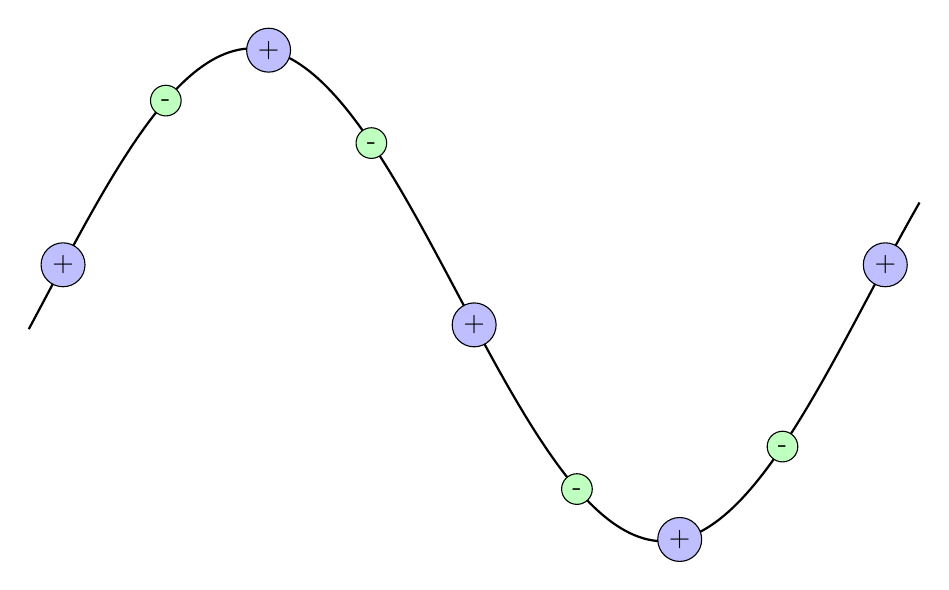
\begin{tikzpicture}[]
            \begin{axis}[
                  axis x line=none,
                  axis y line=none,
                  domain=-195:195,
                  samples=201,
                  xticklabels=\empty,
                  width=1.25\linewidth,
                  height=0.75\linewidth
                ]
               \addplot [black, thick] {sin(x + \phase)};
               \node[shape=circle,fill=blue!25,draw,inner sep=2pt] at (axis cs:-180,{sin(-180 + \phase)}) {+};
               \node[shape=circle,fill=green!25,draw,inner sep=2pt] at (axis cs:-135,{sin(-135 + \phase)}) {-};
               \node[shape=circle,fill=blue!25,draw,inner sep=2pt] at (axis cs:-90,{sin(-90 + \phase)}) {+};
               \node[shape=circle,fill=green!25,draw,inner sep=2pt] at (axis cs:-45,{sin(-45 + \phase)}) {-};
               \node[shape=circle,fill=blue!25,draw,inner sep=2pt] at (axis cs:0,{sin(0 + \phase)}) {+};
               \node[shape=circle,fill=green!25,draw,inner sep=2pt] at (axis cs:45,{sin(45 + \phase)}) {-};
               \node[shape=circle,fill=blue!25,draw,inner sep=2pt] at (axis cs:90,{sin(90 + \phase)}) {+};
               \node[shape=circle,fill=green!25,draw,inner sep=2pt] at (axis cs:135,{sin(135 + \phase)}) {-};
               \node[shape=circle,fill=blue!25,draw,inner sep=2pt] at (axis cs:180,{sin(180 + \phase)}) {+};
        	\end{axis}
        \end{tikzpicture}
        \subcaption{Akustische Mode}
    \end{subfigure}
    \begin{subfigure}[t]{0.48\linewidth}
        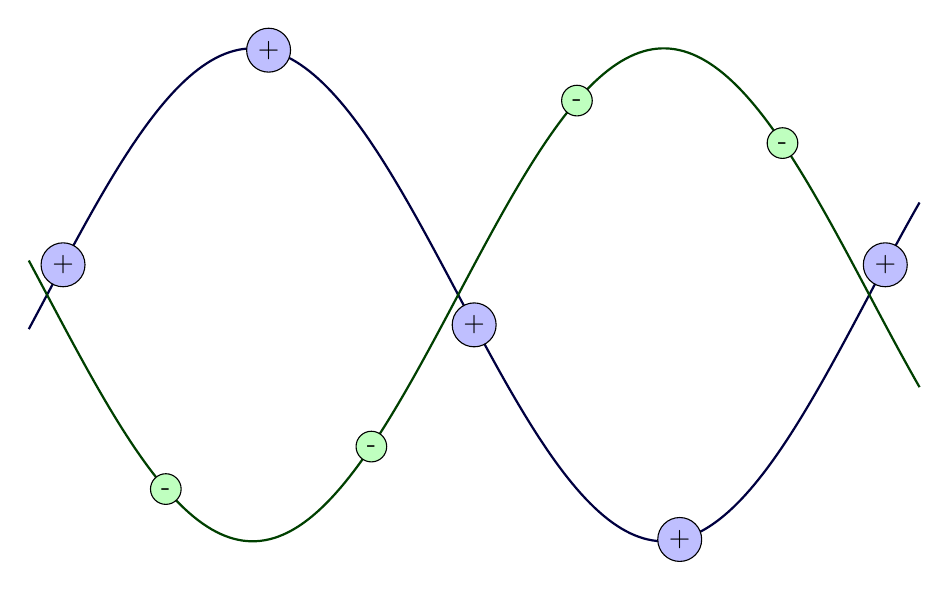
\begin{tikzpicture}[]
            \begin{axis}[
                  axis x line=none,
                  axis y line=none,
                  domain=-195:195,
                  samples=201,
                  xticklabels=\empty,
                  width=1.25\linewidth,
                  height=0.75\linewidth
                ]
               \addplot [blue!25!black, thick] {sin(x + \phase)};
               \addplot [green!25!black, thick] {sin(x + \phase + 180)};
               \node[shape=circle,fill=blue!25,draw,inner sep=2pt] at (axis cs:-180,{sin(-180 + \phase)}) {+};
               \node[shape=circle,fill=green!25,draw,inner sep=2pt] at (axis cs:-135,{sin(-135 + \phase + 180)}) {-};
               \node[shape=circle,fill=blue!25,draw,inner sep=2pt] at (axis cs:-90,{sin(-90 + \phase)}) {+};
               \node[shape=circle,fill=green!25,draw,inner sep=2pt] at (axis cs:-45,{sin(-45 + \phase + 180)}) {-};
               \node[shape=circle,fill=blue!25,draw,inner sep=2pt] at (axis cs:0,{sin(0 + \phase)}) {+};
               \node[shape=circle,fill=green!25,draw,inner sep=2pt] at (axis cs:45,{sin(45 + \phase + 180)}) {-};
               \node[shape=circle,fill=blue!25,draw,inner sep=2pt] at (axis cs:90,{sin(90 + \phase)}) {+};
               \node[shape=circle,fill=green!25,draw,inner sep=2pt] at (axis cs:135,{sin(135 + \phase + 180)}) {-};
               \node[shape=circle,fill=blue!25,draw,inner sep=2pt] at (axis cs:180,{sin(180 + \phase)}) {+};
        	\end{axis}
        \end{tikzpicture}
        \subcaption{Optische Mode}
    \end{subfigure}
    \caption{Phononenmoden der zweiatomigen Basis}
    \label{fig:phononenmoden}
\end{figure}


\begin{fquestion}{Wie äußern sich die Moden bei einer zweiatomigen Basis?}
    Ein Vergleich von optischen und akustischen Transversalwellen von Phononen bei 2-atomiger Basis für kleine $k$ ist in \autoref{fig:phononenmoden} dargestellt.
    \\
    Für $|k|\rightarrow \frac{\pi }{a}$ schwingt jeweils nur eine Atomsorte, wobei $\omega_+ = \sqrt{\frac{2C}{m}}$ und $\omega_- = \sqrt{\frac{2C}{M}}$ ist ($M > m$).
    Die Wellenlänge ist jeweils $\lambda = \frac{2\pi }{k} = 2a$.
\end{fquestion}

\begin{fquestion}{Was ist die Laue-Bedingung?}
    Die Impulsänderung $\Delta\Vec{k} = \Vec{k}_\mathrm{out} - \Vec{k}_\mathrm{in}$ muss einem reziproken Gittervektor $\Vec{G}$ entsprechen.
\end{fquestion}

\subsection{Magnonen}

\begin{figure}[ht!]
    \centering
    \animategraphics[autoplay, width=0.5\textwidth,loop]{15}{img/spin_wave/Spin_wave-}{1}{2}
    \caption{Animation einer Anregung in der Mitte eines Spin-Feldes. Die Anregung propagiert durch den Drehmomente und damit den Austausch von Drehimpuls.
    \refimgsource{Wikimedia}{https://commons.wikimedia.org/wiki/File:Spin_wave.gif}{18.01.2022}{public domain}}
\end{figure}

\begin{fquestion}{Was sind Magnonen?}
    Magnonen sind bosonische Quasiteilchen; sie treten bspw. in Festkörpern als quantisierte Spinwellen auf (analog zum Phonon als quantisierte Schallwelle).
\end{fquestion}

\begin{fquestion}{Wie ist die Dispersionsrelation der Magnonen?}
    Für Magnonen im Ferromagneten gilt die Dispersionsrelation 
    \[ \hbar \omega = 4 J S (1 - \cos a k) \approx 2 J S a^2 k^2 := D k^2 \]
    mit $D = 2 J S a^2 \approx \SI{281}{\milli\electronvolt\angstrom\squared}$, wobei $J$ die Kopplungskonstante, $S$ der Betrag des Spins und $a$ die Gitterkonstante sind.
\end{fquestion}


% \begin{question}{Warum ist die Kurve der Dispersionsrelation am Rand der Brillouin Zone abgeflacht? }
%     Welle wird am Rand der BZ reflektiert und es bildet sich eine stehende Welle, Gruppengeschwindigkeit 0 und daher die Ableitung der Dispersionrelation auch Null
% \end{question}

% \begin{question}{Was sind die masselosen und massiven Anregungen des Systems?}
%     Im Potential gezeigt, dass masselos (Nambu-Goldstone-Anregung) entlang Kreis im Hut-Potential (also 3D-Doppelmuldenpotential) ohne Änderung der potentiellen Energie und massiv (Higgs-Anregung) "entlang Potentialwände"
% \end{question}


% \begin{question}{Was stellen die Anregungen allgemein dar?}
%     einmal Fluktuation ohne betraglicher Änderung des OP, einmal mit
% \end{question}

\begin{fquestion}{Was ist der Unterschied zwischen massiven und masselosen Spinwellen?}
    Die massiven Magnonen sind lokale Störungen der Magnetisierung, die sich wellenartig ausbreiten können ($\si{\micro\electronvolt}$).
    Die masselosen Anregungen ($\lambda = \infty$) beschreiben Spindrehung des gesamten Ferromagneten ohne betraglicher Änderung der Magnetisierung.
\end{fquestion}

\begin{fquestion}{Was passiert mit einzelnen Spins bzw. den Anregungen nahe der kritischen Temperatur?}
    Knapp unterhalb der kritischen Temperatur ist die Wahrscheinlichkeit sich parallel zu den benachbarten Momenten auszurichten etwas größer als die einer willkürlichen Ausrichtung. 
    Oberhalb der kritischen Temperatur ist es entsprechend andersherum.
\end{fquestion}

% \begin{question}{Wie kann man die Anregungen vermessen?}
%     Inelastische Neutronenstreuung, kurz bisschen was dazu erzählt ???
% \end{question}

% \begin{question}{Wie kann man denn so ein Magnon unendlicher Wellenlänge verstehen? }
%     Spindrehung des gesamten Ferromagneten, d.h. alle Spins drehen sich kollektiv in eine Richtung 
    
%     Betrag der Magnetisierung ändert sich nicht, nur die Richtung
% \end{question}

\begin{fquestion}{Wie kann man Magnonen messen?}
    Durch Neutronenstreuung: Das magnetische Moment des Neutron ($\mu_n = \frac{e \hbar}{2 m_p}$, entsteht durch die Konstituentenquarks) wechselwirkt mit den magnetischen Momenten der Elektronen und entsprechend kann man deren Verteilung messen.
    In Kernreaktoren oder dur Spallationsquellen (Beschuss von Atomkernen mit schnellen $> \SI{100}{\mega\electronvolt}$ Projektilen) können schnelle Neutronen freigesetzt werden.
    Da das magnetische Moment des Neutron viel kleiner als dessen Masse ist, müssen die Neutronen vorher abgebremst werden, damit die Wechselwirkung mit den Magnonen überhaupt beobachtet werden kann.
    
    Auf anderem Weg können Magnonen über Experimente mit dünnen Ferromagneten und hochfrequenten Magnetfeldern bestimmt werden.
\end{fquestion}

% \begin{question}{Wo kommt das magnetische Moment des Neutrons her? }
%     Unterstruktur der Valenzquarks führt zu $\mu = g_n \mu_{\mathrm{Kern}} S$
% \end{question}

% \begin{question}{Was sind Quellen von Neutronen? }
%     Reaktor oder Spallationsquelle, müssen aber üblicherweise noch abgebremst werden ???    
% \end{question}

\subsection{Festkörper}

\begin{fquestion}{Wie kommt der elektrische Widerstand im Festkörper zustande?}
    Die elektrische Leitfähigkeit ist durch
    $$\sigma = \frac{n e^2 \lambda_F}{m^\star v_F}$$
    gegeben, wobei $n$ die Elektronendichte, $\lambda_F$ die mittlere freie Weglänge für Elektronen mit Fermi-Energie, $m^\star$ die reduzierte Masse und $v_F$ die Fermi-Geschwindigkeit sind.
    
    Phänomenologisch entsteht der elektrische Widerstand durch die Streuung von Elektronen an den Phononen des Kristallgitter (deren An- bzw. Abregung) und an Störstellen im Kristall bei ihrer thermischen Geschwindigkeit.
    Eine Streuung an anderen Elektronen oder Atomrümpfen findet selten statt.
\end{fquestion}


\begin{fquestion}{Wie sieht die Dispersionsrelation für Elektronen aus?}
    Die Dispersionsrelation für Elektronen ist quadratisch $E \propto k^2$, durch das Entstehen von stehenden Wellen am Rand der Brillouin-Zone flacht diese dort ab. 
    Die entsprechende Bandstruktur kann durch das Umklappen der Dispersionsrelationen am Rand der Brillouin-Zone erhalten werden:
    \begin{center}
        \includegraphics[width=0.7\linewidth]{img/32672_5_De_13_Fig13_HTML.png}
    \end{center}
    
    \refimgsource{Elektronen im Festkörper}{https://media.springernature.com/lw785/springer-static/image/chp\%3A10.1007\%2F978-3-662-49094-5_13/MediaObjects/32672_5_De_13_Fig13_HTML.gif}{14.02.2022}{Keine}
\end{fquestion}
    
\begin{fquestion}{Was passiert, wenn sich zwei Elektronenbänder kreuzen?} 
    Beim Kreuzen zweier Energiebänder wären die Zustände eigentlich entartet, physikalisch entspricht diese Situation zwei stehenden Wellen mit gleicher Wellenlänge und Frequenz.
    Im Festkörper findet allerdings eine zusätzliche Auszeichnung durch die Phase beider Wellen statt.
    Entweder ist die Phase so, dass die Aufenthaltswahrscheinlichkeit ihr Minima genau bei oder entsprechend genau zwischen den Atomrümpfen hat, wodurch sich im ersten Fall eine stärkere Bindung als im zweiten Fall einstellt.
    Entsprechend entsteht eine Bandlücke.
    
    (Argumentation der vermiedenen Kreuzung eventuell auch über den effektiven Massetensor)
\end{fquestion}

\begin{fquestion}{Wie bestimmt man die Zustandsdichte?}
    Allgemein definiert man die Zustandsdichte über
    $$D(E) := \int_{\mathbb{R}^d} \delta(E - E_{\Vec{k}})\,\frac{\mathrm{d}^dk}{(2\pi)^d}, $$
    wobei $d$ die Dimension ist.
    Mit $E=\frac{k^2}{2m}$ und bei Vernachlässigung von Spins ergibt sich daraus dann 
    $$D(E) = \frac{1}{(2\pi)^d }\int_0^\infty \delta \left( E - \frac{k^2}{2m} \right)\, \underbrace{\frac{d\pi^{d/2}k^{d-1}}{\Gamma \left(\frac{d}{2} + 1\right) }}_{\text{Kugeloberfläche}} \,\mathrm{d}k.$$
    Da $\delta \left( E - \frac{k^2}{2m} \right) \equiv \frac{\delta (k-\sqrt{2mE})}{|k/m|}$ ist, folgt letztlich
    $$D(E) = \frac{d\pi^{d/2}(2mE)^{\frac{d-1}{2}}}{(2\pi)^d \Gamma \left(\frac{d}{2} + 1\right)} \frac{m}{\sqrt{2mE}} \propto (2mE)^{\frac{d}{2} - 1} \equiv k^{d-2}.$$
    % Die Zustandsdichte ist definiert als $D(E) := \frac{\mathrm{d}N}{\mathrm{d}E}$, woraus
    % $$N = \int_0^{E_F} D(E) \,\mathrm{d}E = \int_{\mathbb{R}^3} Z(\Vec{k}) \mathrm{d}^3k$$
    % mit der mikrokanonischen Zustandssumme $Z(\Vec{k})$ im Impulsraum durch $$Z(\Vec{k}) = \underbrace{2\cdot}_{\mathrm{Spins}} \frac{V}{(2\pi)^3}$$
    % gegeben.
    % Daraus folgt dann über $E=\frac{k^2}{2m}$ auch 
    % $$\mathrm{d}N = D(E)\, \mathrm{d}E = \frac{2V}{(2\pi)^3} 4\pi k^2\,\mathrm{d}k = \frac{8\pi Vk^2}{(2\pi)^3} \frac{1}{2} \sqrt{\frac{2m}{E}} \,\mathrm{d}E,$$
    % also $D(E) = \frac{mV}{\pi^2}\sqrt{2mE}$.
    
\end{fquestion}

\begin{fquestion}{Wie hängen Fermi-Impuls $k_F$ und die Spin-$\frac{1}{2}$-Fermionendichte zusammen?}
    Es ist $n=\frac{N}{V} = \frac{1}{V} \cdot \frac{V}{(2\pi)^3}\cdot \frac{4\pi}{3}k_F^3 = \frac{k_F^3}{6\pi^2}$ die Besetzungszahldichte.
    Da jeder Zustand von zwei Fermionen besetzt werden kann, ist $n_{1/2} = 2n$.
    Also gilt $k_F = \sqrt[3]{3\pi^2 n_{1/2}}$.
\end{fquestion}

\begin{fquestion}{Wie könnte man diesen Ausdruck für einen symmetrischen Kern noch vereinfachen?}
    Symmetrisch bedeutet hier $N=Z=\frac{A}{2}$.
    Mit $V\simeq \frac{4\pi}{3} R^3$ und $R\simeq R_0 A^{1/3}$ folgt dann 
    $$k_F \simeq \sqrt[3]{3\pi^2 \frac{A}{\frac{4\pi}{3}R_0^3 A}} = \frac{3}{2R_0}\sqrt[3]{\frac{2\pi}{3} }.$$
    Insbesondere gilt für den Fermi-Impuls der Protonen bzw. Neutronen dann $k_F^{\text{p}/\text{n}} = \frac{3}{2R_0}\sqrt[3]{\frac{\pi}{3} }$, weil nur die halbe Nukleonenzahl $\frac{A}{2}$ in die ``Gesamtanzahl'' an Fermionen eingeht.
\end{fquestion}

\begin{fquestion}{Wie könnte man damit grob die Fermi-Energie von Kernen abschätzen?}
    Die Fermi-Energie ist etwa $E_F=\frac{k_F^2}{2m} \simeq \frac{9}{8mR_0^2} \left(\frac{\pi}{3}\right)^{2/3}$.
    Für einen (symmetrischen) Kern gilt mit $R_0 \approx \SI{1.2}{fm}$ also 
    $$E_F \approx \frac{9\cdot (\SI{200}{MeV\femto\metre})^2}{8\cdot \SI{1000}{MeV} \cdot (\SI{1.2}{fm})^2 } \cdot 1.03 \approx \SI{32}{MeV}. $$
\end{fquestion}

\begin{fquestion}{Wie würde man die Fermi-Energie von einem Gold-Atom und einem weißen Zwerg abschätzen?}
    Allgemein gilt $E = \frac{k_F^2}{2m} = \frac{1}{2m} \left( 3\pi^2 n_{1/2} \right)^{2/3}$, man muss also die Masse und die Fermionendichte abschätzen.
    \\
    Gold liegt üblicherweise in einem fcc-Gitter vor, es gibt also $8\cdot \frac{1}{8} + 6\cdot\frac{1}{2} = 4$ Atome pro Zelle.
    Unter der Annahme, dass jeweils ein Elektron pro Atom frei ist, und dass die Kantenlänge $a$ der Zelle etwa $2\sqrt{2} r_0$ ist (Atome berühren sich auf der Diagonalen), folgt dann $k_F = \sqrt[3]{3\pi^2 \frac{4}{a^3}} \approx \SI{2}{keV}$ (Radius von Gold ist $r_0\approx \SI{166}{pm}$).
    Die Fermi-Energie ist somit $E_F \approx \frac{(\SI{2}{keV})^2}{2\cdot \SI{0.5}{MeV}} = \SI{4}{eV}.$
    \\
    Im Stern können wir annehmen, dass (fast) alle Elektronen frei sind, also ist 
    $$N_{1/2} \approx 26\cdot \frac{m_\mathrm{Stern}}{m_\mathrm{Fe}} \approx 26\cdot \frac{\SI{2e30}{kg}}{56m_n} \approx \SI{3e56}.$$
    Das Volumen ist $V = \frac{4\pi }{3} R_\mathrm{Stern}^3 \approx \SI{1.4e21}{m^3}$ ($R_\mathrm{Stern} \approx \SI{7e6}{m}$, also etwa 1\,\% des Sonnenradius).
    Der Fermi-Impuls ist damit $k_F \approx \sqrt[3]{3\pi^2 \frac{N_{1/2} }{V}} \approx \SI{1.8e12}{m^{-1}}$.
    Die Fermi-Energie folgt dann zu $E_F \approx \SI{0.13}{MeV}$.
    Das ist von dem tatsächlichen Wert von $0.3\,$MeV allerdings deutlich entfernt, die Abschätzung ist dafür viel zu ungenau.
\end{fquestion}

\begin{fquestion}{Warum tragen die Eisen-Kerne nicht zur Fermi-Energie bei?}
    Die Eisen-Kerne sind Bosonen, da ${}^{56}_{26}\mathrm{Fe}$ gerade Proton- und Neutronzahl hat, der Spin ist also ganzzahlig.
\end{fquestion}

\begin{fquestion}{Welches Kopplungsschema ist wann relevant?}
    LS: Die Coulomb-Abstoßung der Elektronen ist groß gegenüber der Spin-Bahn-Wechselwirkung, also gilt näherungsweise $$\begin{aligned}\Vec{L} &= \sum \Vec{l}_k, && \mathrm{und} & \Vec{S} &= \sum \Vec{s}_k\end{aligned}.$$
    Der Gesamtdrehimpuls ist dann $\Vec{J} = \Vec{L} + \Vec{S}$.
    Das gilt meist für leichte Kerne ($Z\lesssim 30$).
    \\
    jj: Die Spin-Bahn-Wechselwirkung groß gegenüber der Coulomb-Abstoßung, also können sich $\Vec{l}_k$ und $\Vec{s}_k$ nicht mehr unabhängig voneinander ausrichten.
    Phänomenologisch kann man argumentieren, dass durch $\Delta E_{LS} \sim \langle \Vec{l}\cdot\Vec{s} \rangle$ der ``Winkel'' zwischen den Vektoren ``fest'' ist.
    Dann koppeln die einzelnen Drehimpulse zu $\Vec{j}_k = \Vec{l}_k + \Vec{s}_k$, und es gilt dann
    $$\Vec{J} = \sum \Vec{j}_k.$$
    Das tritt vor allem für schwere Kerne auf ($Z\gtrsim 30$).
    
    Beides sind aber nur Näherungen. 
    Insbesondere tritt jj-Kopplung beispielsweise auch bei starken externen Magnetfeldern auf (siehe Paschen-Back-Effekt).
\end{fquestion}

\begin{fquestion}{Wie kann die Spin-Bahn-WW noch überwunden werden?}
    Mit einem externen Magnetfeld, siehe auch Zeeman- bzw. Paschen-Back-Effekt.
\end{fquestion}

\begin{fquestion}{Was besagen die Hund'schen Regeln?}
    Es ist derjenige elektronische Zustand mit maximalem Gesamtspin $S$ bevorzugt.
    Falls mehrere Zustände möglich sind, soll auch der Bahndrehimpuls $L$ maximal sein.
    Die Regeln beruhen auf der Coulomb-Abstoßung und maximieren (näherungsweise) den mittleren Abstand zwischen den Elektronen, und minimieren damit die Energie.
\end{fquestion}

\begin{fquestion}{Wie werden d-Orbitale von 6 Elektronen besetzt?}
    Es gibt $2(2l + 1) = 10$ Orbitale ($2l+1$ verschiedene $m_L$ und je zwei $m_S$), von denen 6 besetzt werden sollen.
    Nach den Hund'schen Regeln verteilen wir die ersten 5 Elektronen so, dass alle parallelen Spin haben. 
    Das letzte Elektron hat dann entsprechend umgekehrten Spin, und besetzt das $m_L=2$-Orbital, also $S=2$.
    Damit ist der Spin $S= \frac{1}{2}(5 - 1) = 2$ und der Bahndrehimpuls $L=2$, also $J = 0\dots 4$.
\end{fquestion}

\begin{fquestion}{Warum ist es kein Widerspruch, dass die Elektronen bei LCAO bevorzugt zwischen den Kernen sind und im Festkörper bevorzugt an den Kernen?}
    Beide Phänomene haben ihren Ursprung in der LCAO- bzw. Tight-Binding-Methode.

    Bei der LCAO-Methode wird die Orbitalstruktur von Molekülen untersucht; dabei gilt die Annahme dass sich die gemeinsame Molekülorbitalstruktur aus den Atomorbital zusammensetzt. 
    Beim Wasserstoff entsteht hierbei ein symmetrischer und ein anti-symmetrischer Grundzustand, wobei nur der symmetrische Zustand zu einer energetisch günstigen Bindung führt.
    Die beiden Elektronen des Wasserstoff sind also symmetrisch gebunden, wobei der symmetrische Zustand eine nicht verschwindende Aufenthaltswahrscheinlichkeit zwischen den Kernen hat.
    
    Beim Festkörper betrachten wir quasi-freie Elektronen, die schwach mit dem Kristallgitter wechselwirken. 
    Für ein einzelnes Elektron wird wieder das Atomorbital lokalisiert einem Gitterplatz als Wellenfunktion beibehalten.
    Durch die anderen Gitterplätze kommt es zu mehreren wichtigen Matrixelementen:
    \begin{itemize}
        \item Der (meist kleinen) Absenkung der Eigenenergie durch das Potential der anderen Gitterplätze,
        \item dem Bindungsterm (der den Potentialerwartungswert des Überlapps zweier Elektronen an verschiedenen Gitterplätzen beschreibt) und
        \item dem Überlappterm.
    \end{itemize}
    Durch die Form des Gitters ist es nun energetisch günstig sich bei einem Atomrumpf zu positionieren. 
    Nach dem Bloch-Theorem muss sich die Wellenfunktion um die Gitterkonstante verschieben lassen, bei einem stark-bindenden Festkörper würden zwischen den Rümpfen lokalisierte Elektronen also weniger stark gebunden sein als bei den Rümpfen gebundene.
    Die Potentialreichweite der Rümpfe ist klein, ergo ist der Verlust beim Überlapp mit dem eigenen Atomrumpf so gravierend dass er nicht durch den zusätzlichen Überlapp mit dem benachbarten Atomrumpf kompensiert werden kann.

    % bei LCAO für Bindung verantwortlich, im FK sind sie quasifrei ??? 
    Dass beim Wasserstoff die Bindung mit Lokalisierung des Elektrons zwischen den beiden Kernen und beim Festkörper die Lokalisierung des Elektrons bei den Atomrümpfen energetisch günstiger sind folgt anschaulich also jeweils aus der Symmetrie des Problems. 
\end{fquestion}
